\newpage
\section*{\LARGE{Глава 4. Построение оптимальной сети}}
\addcontentsline{toc}{section}{Глава 4. Построение оптимальной сети}
\hskip 12 mm
После того как мы научились находить оптимальные пути между двумя точками, стоит задача построения оптимальной сети линейных объектов. Встречаемые в литературе алгоритмы построение деревьев Штейнера на графах ориентированы на более общий случай задачи, поэтому будут недостаточно эффективны в нашем случае. Граф в нашем случае является сильно разреженным, с малым числом терминальных вершин, относительно общего количества вершин в графе, а также наша задача является прикладной. Поэтому было решено разработать собственный алгоритм, использующий определенную эвристику для эффективного построения оптимальной сети.
\subsection*{\Large{4.1 Описание используемого алгоритма}}
\addcontentsline{toc}{subsection}{4.1 Описание используемого алгоритма}
\hskip 12 mm
Введем ряд определений, используемых далее.

Пусть задан граф $\mathbb{G} = (\mathbb{V}_G, \mathbb{E}_G)$, где $ \mathbb{V}_G = \{v_1, v_2, ..., v_n\}$ --- множество вершин, а $ \mathbb{E}_G = \{e_1, e_2, ..., e_m\}$ --- множество рёбер.

Терминальными точками назовем множество точек  $T \subseteq  \mathbb{V}_G$, между которыми требуется построить дерево Штейнера.

При этом такой подграф $ST \subseteq \mathbb{G}$, соединяющий $T$, минимально возможного веса $w(ST)$ является деревом, которое называется минимальным деревом Штейнера на $T$.

Точками Штейнера называется множество точек $P \subseteq \mathbb{V}_{ST} \textbackslash T$.

Точками разветвления назовем подмножество точек Штейнера $S \subseteq P$, которые были добавлены во время работы алгоритма, реализующие лучшее решение, чем построенное только на терминальных точках.

Минимальное остовное дерево --- это остовное дерево этого графа, имеющее минимальный возможный вес, где под весом дерева понимается сумма весов, входящих в него рёбер \cite{MST}. Обозначим сумму весов ребер графа за  
$w: \mathbb{G} \rightarrow \mathbb{R}$.
\subsection*{\Large{Идея алгоритма}}
\hskip 12 mm
Для начала, создается ограничительный прямоугольник, для которого мы генерируем набор точек разветвления. Мы разбиваем прямоугольник на $n_x$ точек по горизонтали и $n_y$ точек по вертикали. Итого, имеем $n_x \cdot n_y$  точек разветвления на плоскости (см. рис. \ref{pic:get_steiner_nodes}). Для каждой точки разветвления мы находим ближайшую к ней по расстоянию вершину в графе.

\begin{figure}[H]
	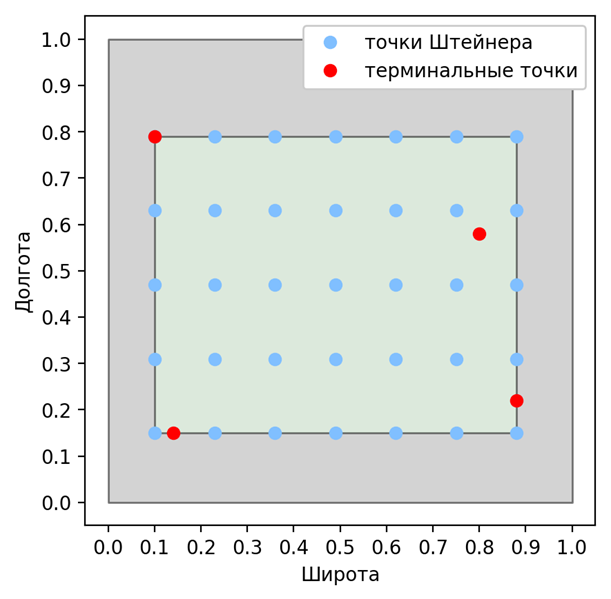
\includegraphics[width=0.7\textwidth]{images/4_1.png}
	\caption{Получение точек Штейнера}
	\label{pic:get_steiner_nodes}
\end{figure}
\vskip 4mm
После получения набора точек разветвления, нам нужно выбрать такое их подмножество, которое образует дерево минимального веса (см. рис. \ref{pic:get_MST}). Для этого нам потребуется вычислять минимальные остовные деревья (далее $MST$).

\begin{figure}[H]
	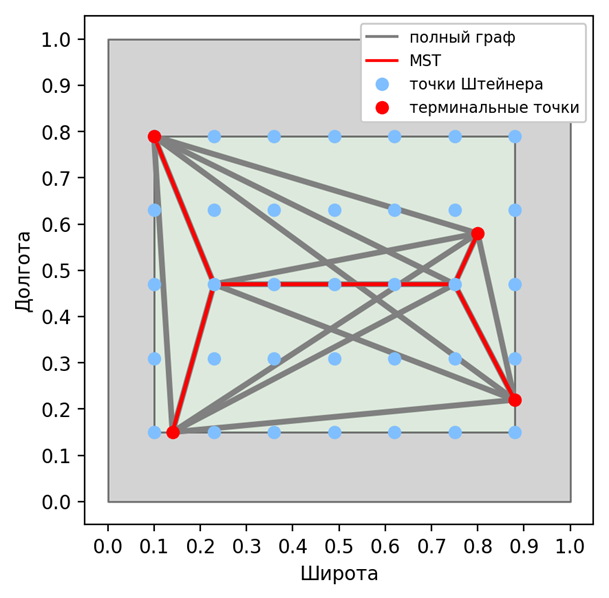
\includegraphics[width=0.7\textwidth]{images/4_2.png}
	\caption{Полный граф и MST}
	\label{pic:get_MST}
\end{figure}
\vskip 4mm

Известно, что количество точек разветвления в итоговом графе не может превышать $m = |T| - 2$, где $|T|$ - количество терминальных точек. Соответственно, наш алгоритм будет иметь $m$ шагов. Создадим массив $step\_solutions$, отвечающий за хранение $k$ лучших результатов, полученных на каждом шаге алгоритма.

На каждой итерации алгоритма нам требуется построить набор полных графов для различных комбинаций терминальных точек и точек разветвления. Этот этап можно выделить в функцию get\_full\_graphs. Набор полных графов строится по следующему принципу: за основу для генерации берется набор терминальных точек,  Весами ребёр в полном графе будет стоимость кратчайшего пути между двумя вершинами ребра в изначальном графе. То есть, пусть у нас задано $t = |T|$ терминальных точек, $k$ лучших решений и $n$ точек разветвления, таким образом у нас должно быть сгенерировано $k \cdot n$ полных графов, так как терминальные вершины добавляются всегда, как и наборы вершин из лучших решений. И к каждому из этих наборов вершин нужно добавить по одной из точек разветвления.

После этого для каждого полученного полного графа требуется построить минимальное остовное дерево и взвесить его.

Далее нужно отобрать $k$ лучших по весу минимальных остовных деревьев и добавить их в массив $step\_solutions$, отвечающий за лучшие решения на текущем шаге.

После того, как все шаги выполнены, нужно найти минимальное по весу дерево среди всех полученных решений из $step\_solutions$. А далее нам нужно восстановить кратчайшие пути между вершинами полученного решения и таким образом мы получим оптимальную сеть $L_{res}$, состоящую из набора ломаных линий.

Псевдокод данного алгоритма представлен на Algorithm \ref{algo:steiner_tree}.

\begin{algorithm}[H]
	\SetAlgoLined
	\KwData{$\mathbb{G} = (\mathbb{V}_G, \mathbb{E}_G)$ - взвешенный граф, $T \subseteq \mathbb{V}_G$  - набор терминальных точек }
	\KwResult{$L_{res} = \{\{x_{j},y_{j}\}_{j=1}^{n_i}, i=\overline{1..s}\}$ - оптимальная сеть линейных объектов }
	
	$steiner\_nodes$ := generate\_steiner\_nodes($\mathbb{G}$, $T$)\\
	$step\_solutions$ := $\varnothing$\\
	$m$ = $|T|$ - 2\\
	\For{$\textbf{i = } 0 \textbf{ to } m-1$}
	{
		$full\_graphs$ := get\_full\_graphs($T$, $step\_solutions$[i-1], $steiner\_nodes$)\\
		$builded\_MSTs$ := get\_MSTs($full\_graphs$)\\
		$step\_solutions$[i] := k\_best\_MSTs($builded\_MSTs$)		
	}
	
	$best\_solution$ := $min(step\_solutions)$\\
	$result$ := recover\_paths($best\_solution$)

\caption{Алгоритм нахождения оптимальной сети}
\label{algo:steiner_tree}
\end{algorithm}

\subsection*{\Large{4.2 Описание модельных карт для тестирования}}
\addcontentsline{toc}{subsection}{4.2 Описание модельных карт для тестирования}
\hskip 12 mm
Задача данного исследования найти зависимость между параметрами: временем работы программы и точностью получаемого решения. Для проведения этого исследования воспользуемся модельной картой в виде квадрата размером $[1.0 \times 1.0]$ градусов и построим вычислительную сетку с размером $d$ = 250 м. Параметры $n_x$  и $n_y$  будем варьировать в диапазоне $[3, \frac{width}{3d}]$ и $[3, \frac{height}{3d}]$, где $width$ и $height$ – ширина и высота ограничивающего прямоугольника в метрах. Будем строить дерево Штейнера для трех объектов. В качестве эталонного решения, возьмем решение, вычисленное аналитически (см. рис. \ref{pic:steiner_tree_1}).

\begin{figure}[H]
	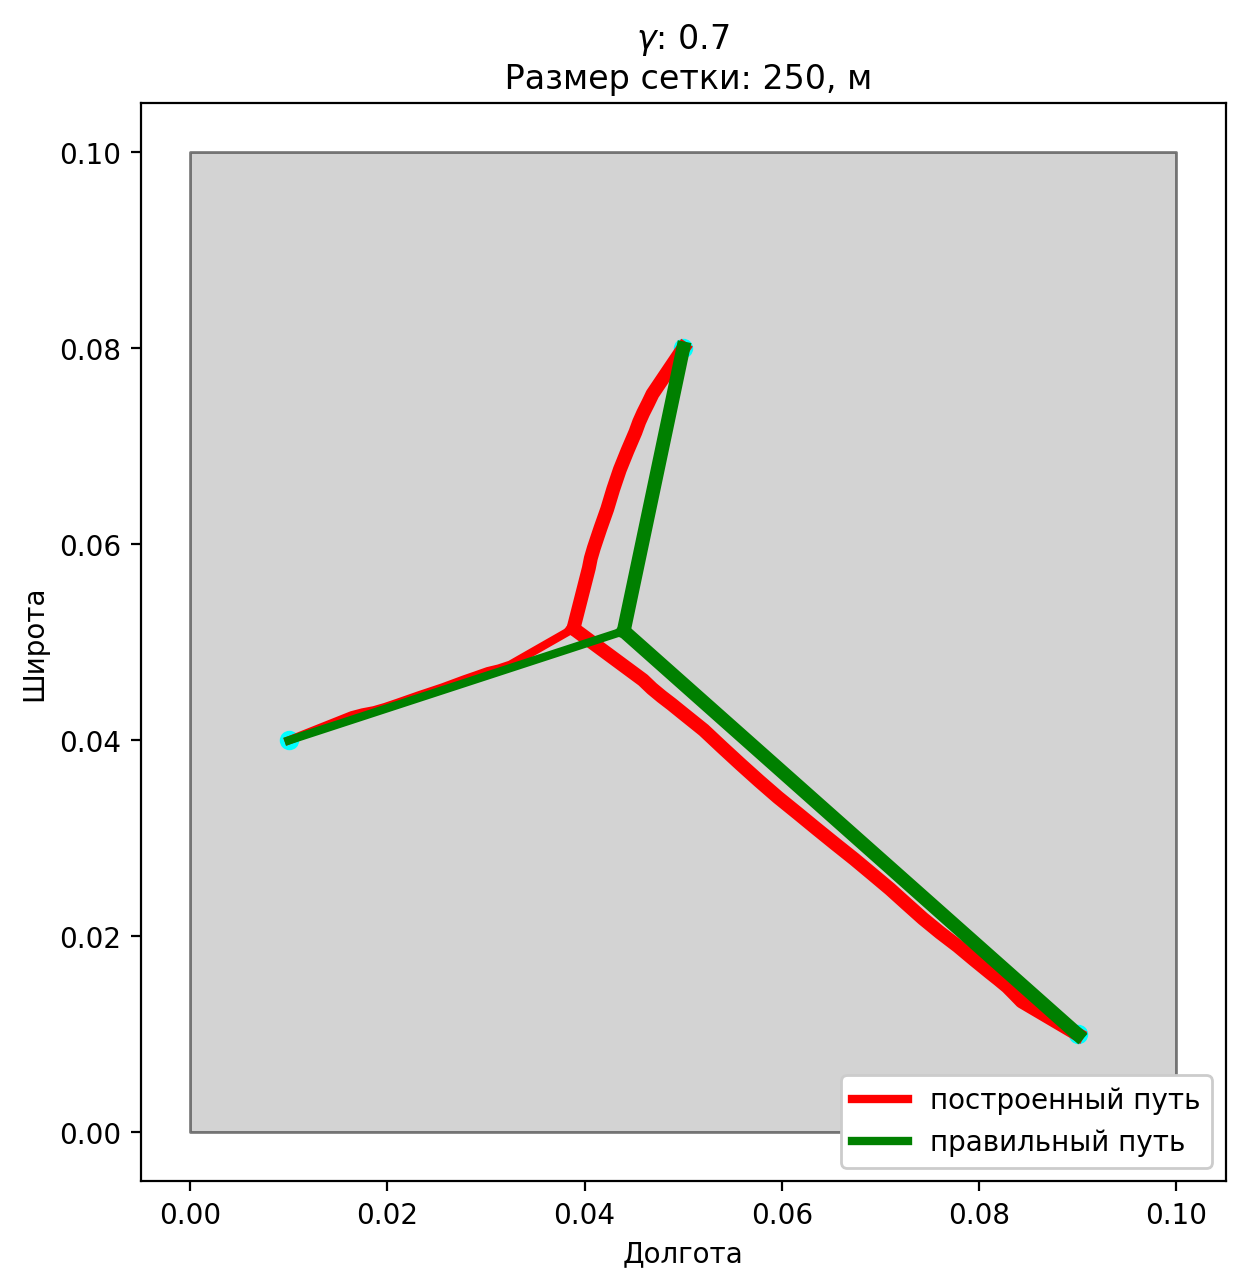
\includegraphics[width=0.7\textwidth]{images/4_3.png}
	\caption{Пример получившегося решения}
	\label{pic:steiner_tree_1}
\end{figure}
\vskip 4mm


После выполнения вычислений была получена следующая таблица(см. табл. \ref{tabular:steiner_res_1}). Всего точек в графе 198025.

\begin{table}[H]
	\centering
	\caption{Результаты работы алгоритма}
	\label{tabular:steiner_res_1}
	\begin{tabular}{|c|c|c|c|c|}
		\hline
		\textbf{Ошибка, \%} & \textbf{Время, сек} & \textbf{Точки разветвления} \\ \hline
		4.812 &	3.0 & 9 \\ \hline
		1.216 &	68.6 &	143 \\ \hline
		0.897 &	125.4 &	480 \\ \hline
		1.061 &	236.3 &	980 \\ \hline
		0.979 &	372.6 &	1702 \\ \hline
		1.017 &	531.4 &	2565 \\ \hline
		0.985 &	665.1 &	3618 \\ \hline
		0.939 &	885.6 &	4836 \\ \hline
		0.855 &	1079.2 & 6319 \\ \hline
		0.924 &	1271.6 & 7900 \\ \hline
		0.912 &	1415.4 & 9768 \\ \hline
	\end{tabular}
\end{table}
\vspace{4mm}

Исходя из данных в этой таблице видно, что на плоскости качественные результаты можно получать при количестве точек разветвления в размере около 0.5-1\% от общего числа точек в ограничивающем прямоугольнике.
\par
Помимо поиска решения в простейшем случае, основанных на Евклидовой метрике, требуется описание тестовых случаев для проверки алгоритма на корректность, опираясь на специфику нашей задачи.
\begin{enumerate}
	\item {
		Квадрат размером [1.0 x 1.0] градусов. Данный тестовый случай характерен тем, что три точки образуют угол в 120°. 
		\begin{figure}[H]
			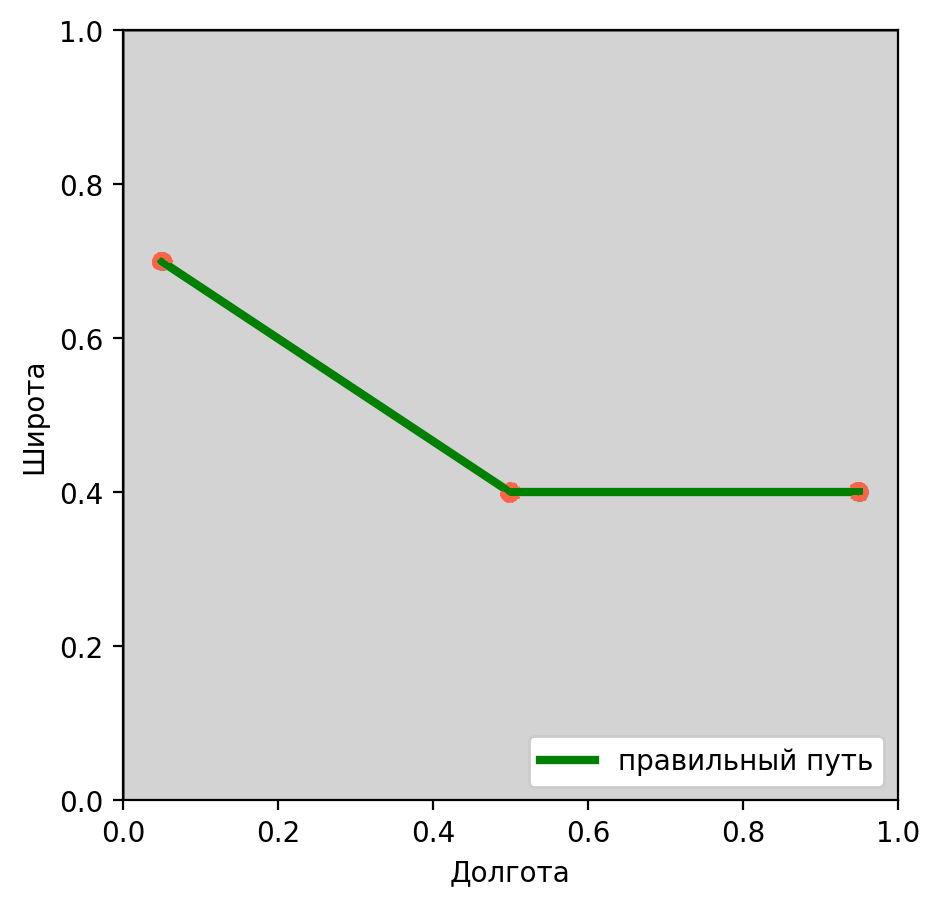
\includegraphics[width=0.5\textwidth]{images/4_4.png}
			\caption{Первый тестовый случай}
			\label{pic:steiner_case_1}
		\end{figure}
		\vspace{2mm}
	}
	\item {
		Квадрат размером [1.0 x 1.0] градусов. Посередине квадрата задана дорога со стоимостью строительства на ней значительно меньшей, чем в окружающей её области. Точка разветвления в этом случае должна находится на дороге. 
		\begin{figure}[H]
			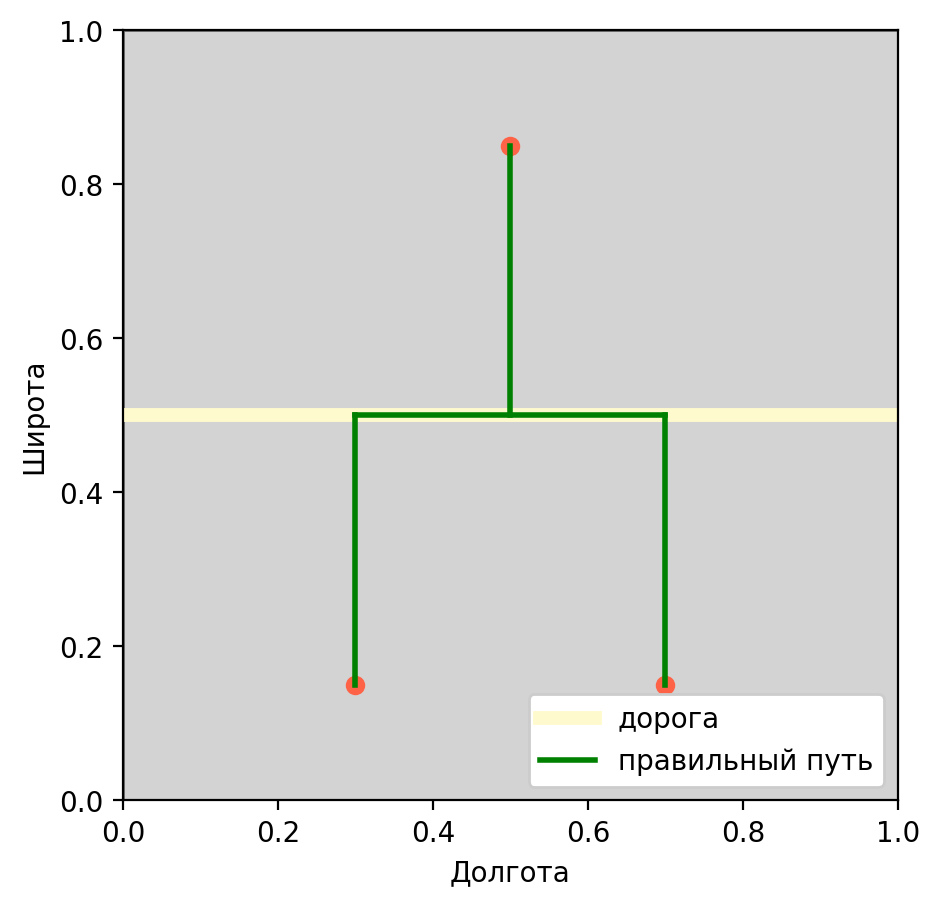
\includegraphics[width=0.5\textwidth]{images/4_5.png}
			\caption{Второй тестовый случай}
			\label{pic:steiner_case_2}
		\end{figure}
		\vspace{2mm}
	}
	\item {
		Квадрат размером [1.0 x 1.0] градусов. В месте, где должна быть точка Штейнера расположена область с высокой стоимостью строительства.
		\begin{figure}[H]
			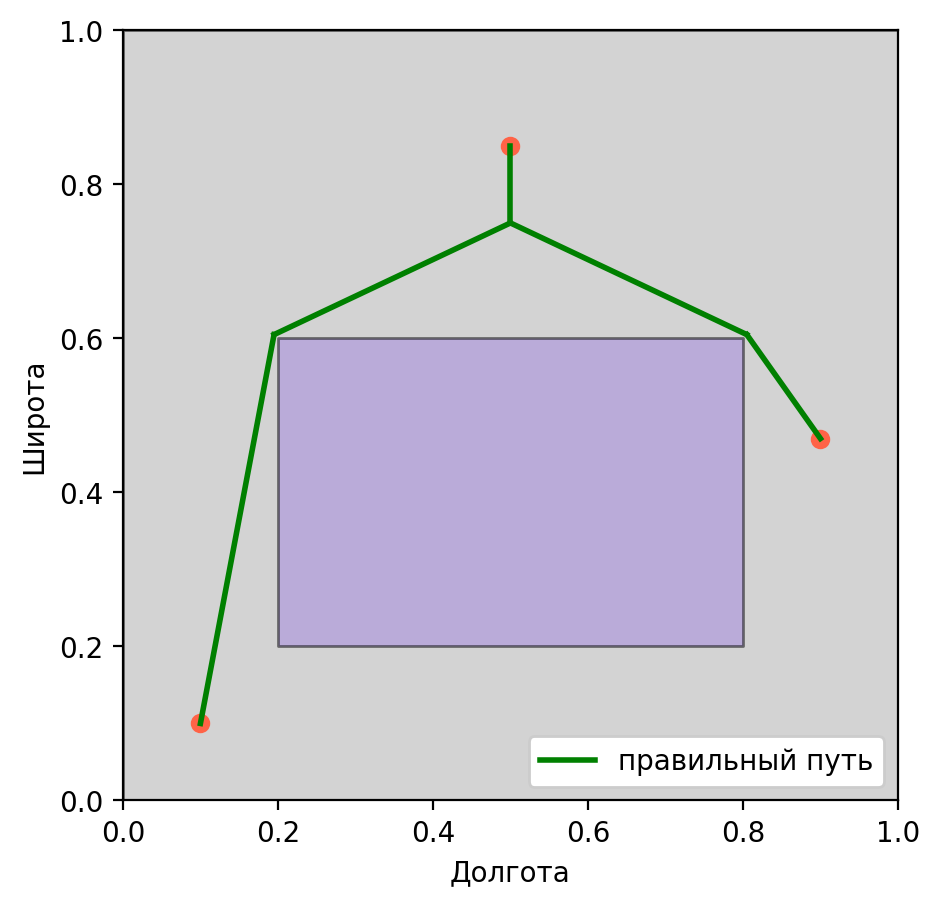
\includegraphics[width=0.5\textwidth]{images/4_6.png}
			\caption{Третий тестовый случай}
			\label{pic:steiner_case_3}
		\end{figure}
		\vspace{2mm}
	}
	\item {
		Квадрат размером [1.0 x 1.0] градусов. Четвертый случай представляет комбинацию предыдущих двух случаев: посередине квадрата проходит дорога с низкой стоимостью строительства на ней, а также на предполгаемом месте точки разветвления находится область с высокой стоимостью строительства.
		\begin{figure}[H]
			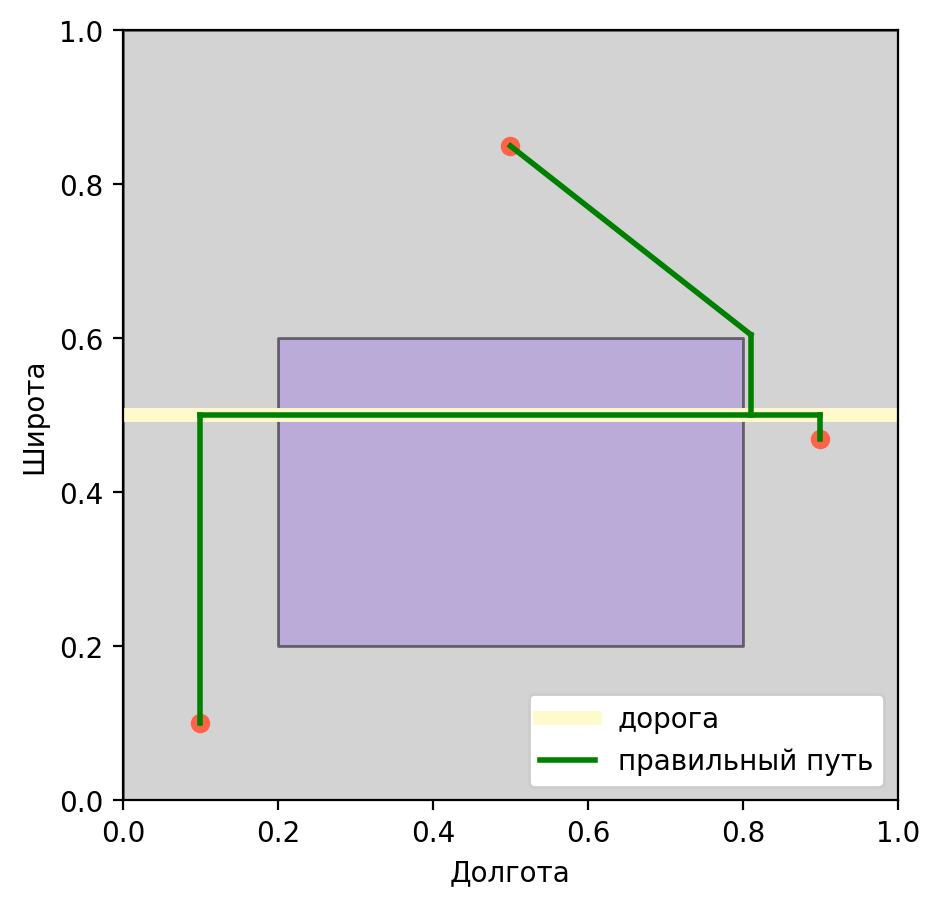
\includegraphics[width=0.5\textwidth]{images/4_7.png}
			\caption{Четвертый тестовый случай}
			\label{pic:steiner_case_4}
		\end{figure}
		\vspace{2mm}
	}
\end{enumerate}
